\documentclass{standalone}
\usepackage{tikz}
\usetikzlibrary{arrows.meta}

\begin{document}
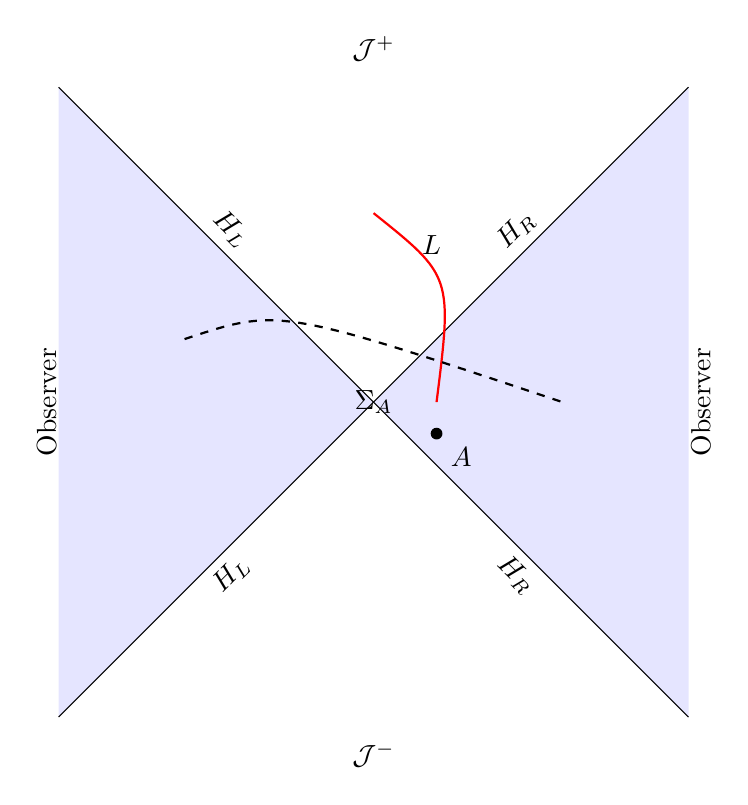
\begin{tikzpicture}[scale=4]

% Define styles
\tikzset{
  event/.style={circle, fill=black, inner sep=1.5pt},
  light/.style={thick, draw=red},
  causal/.style={dashed, thick},
}

% Draw background regions
\fill[blue!10] (0,0) -- (1,1) -- (1,-1) -- cycle;
\fill[blue!10] (0,0) -- (-1,1) -- (-1,-1) -- cycle;

% Draw diagonal boundaries
\draw (0,0) -- (1,1) node[midway, above, sloped] {$H_R$};
\draw (0,0) -- (-1,1) node[midway, above, sloped] {$H_L$};
\draw (0,0) -- (1,-1) node[midway, below, sloped] {$H_R$};
\draw (0,0) -- (-1,-1) node[midway, below, sloped] {$H_L$};

% Draw observer worldlines (causal curves)
\draw[light] (0.2,0) .. controls (0.25,0.4) .. (0,0.6) node[pos=0.8, right] {$L$};
\draw[causal] (-0.6,0.2) .. controls (-0.3,0.3) .. (0.6,0);

% Place event point A
\node[event, label=below right:$A$] (A) at (0.2,-0.1) {};

% Label sigma region
\node at (0,0) {$\Sigma_A$};

% Add observer labels
\node[rotate=90, anchor=south] at (1.1,0) {Observer};
\node[rotate=90, anchor=north] at (-1.1,0) {Observer};

% Add infinity labels
\node[anchor=south] at (0,1.05) {$\mathcal{J}^{+}$};
\node[anchor=north] at (0,-1.05) {$\mathcal{J}^{-}$};

\end{tikzpicture}
\end{document}